\chapter{Interpolation}
\label{Ch: 2-Int}

The interpolation solves problems of the following type:

\begin{quotation}
    Given a set of predefined functions $\cK$, find an element $f: \mathbb{I}\mapsto \bbR$ in $\cK$ such that
    $y_j = f(x_j)$ for all $j=0,\dots, n$.
\end{quotation}
Here, $\mathbb{I}$ denotes a finite or infinite interval such that $x_1,\dots x_n\in \mathbb{I}$. One of the important applications for interpolation is computer-assisted design (CAD), which is used extensively in the manufacturing industry. Generally speaking, the interpolation provides a closed form of the function to determine the value of $y$ where the parameter $x$ is not accessible.

\section{Polynomial Interpolation}
\label{Sec: 2-Pol-Int}
The polynomial interpolation considers the set $\cK = \Pi_m$, where the set $\Pi_m$ represents the polynomials of degree $ \le m$. We will seek for a polynomial $f(x)$ with the constraints that
\begin{equation}\nonumber
    \begin{cases}
        f\in \cK = \Pi_n,&\\
        f(x_k) = y_k &\text{ for } k = 0, 1,\dots, n.
    \end{cases}
\end{equation}
The points $x_k$ are called \emph{interpolation nodes}, if $m > n$ (resp. $m < n$), the problem is underdetermined (resp. overdetermined). For the case that $ m = n$, we have
\begin{theorem}
\label{Thm: 2-Uni-Exi}
    There exists a unique polynomial function $f\in \Pi_n$ such that $f(x_j) = y_j$ for $j=0,\dots, n$.
\end{theorem}
\begin{proof}
   \noindent \emph{Existence: }In order to construct the polynomial $f$, it is straightforward to consider the general form of polynomial $f(x) = \sum_{j=0}^n a_j x^j$, then we can formulate a linear system for the coefficients $a_j$, $j=0,\dots, n$, which is 
    \begin{equation*}
        \begin{pmatrix}
            1 & x_0 & x_0^2 & \dots & x_0^n \\
            1 & x_1 & x_1^2 & \dots & x_1^n \\
            \vdots & \vdots &\vdots & \ddots & \vdots\\
            1 & x_n & x_n^2 & \dots & x_n^n
        \end{pmatrix} \begin{pmatrix}
            a_0\\a_1\\\vdots\\a_n
        \end{pmatrix} = \begin{pmatrix}
            y_0\\y_1\\\vdots \\y_n
        \end{pmatrix}.
    \end{equation*}
    The matrix 
    $$V = \begin{pmatrix}
        1 & x_0 & x_0^2 & \dots & x_0^n \\
        1 & x_1 & x_1^2 & \dots & x_1^n \\
        \vdots & \vdots &\vdots & \ddots & \vdots\\
        1 & x_n & x_n^2 & \dots & x_n^n
    \end{pmatrix} $$
    is called \emph{Vandermonde matrix}.
    To determine the coefficients $a_j$, the matrix $V$ must be invertible. Its determinant can be computed (try to prove it) as
    \begin{eqnarray}
        \det(V) = \prod_{0\le i\le j\le n}(x_j - x_i).
    \end{eqnarray}
    When $\{x_j\}_{j=0}^n$ are distinct, the determinant is nonzero.

   \noindent \emph{Uniqueness: }
    Suppose there are two distinct polynomials $f, g\in \Pi_n$ satisfying the condition that $f(x_j) = g(x_j) = y_j$, then $f - g$ has $(n+1)$ roots $x_j$, $j=0, \dots, n$. If $f\neq g$, it is clear that $f-g\in\Pi_n$ has at most $n$ roots. Contradiction.
\end{proof}

In the above proof, the interpolation polynomial can be uniquely determined by solving the linear system 
$$\begin{pmatrix}
    1 & x_0 & x_0^2 & \dots & x_0^n \\
    1 & x_1 & x_1^2 & \dots & x_1^n \\
    \vdots & \vdots &\vdots & \ddots & \vdots\\
    1 & x_n & x_n^2 & \dots & x_n^n
\end{pmatrix} \begin{pmatrix}
    a_0\\a_1\\\vdots\\a_n
\end{pmatrix} = \begin{pmatrix}
    y_0\\y_1\\\vdots \\y_n
\end{pmatrix}.$$ 
However, it is generally easier to compute the polynomial $f$ with the \emph{Lagrange polynomial interpolation} (which is somewhat equivalent to computing the inverse of $V$).
\subsection{Lagrange Polynomial}
\begin{definition}
    For the given distinct $x_j$, $j = 0, 1, \dots, n$, the $(n+1)$ Lagrange polynomials $L_0, L_1,\dots, L_n\in\Pi_n$ are defined by 
    \begin{equation}
        L_j(x) = \prod_{s = 0, s\neq j}^n \frac{x - x_s}{x_j - x_s}, \quad j = 0, 1,\dots , n.
    \end{equation}
\end{definition}
It is clear that these polynomials satisfy the conditions that 
\begin{equation}
    L_j(x_k) = \delta_{jk} := \begin{cases}
        1&\text{for } k=j,\\
        0&\text{for } k\neq j.
    \end{cases}
\end{equation}
Therefore these polynomials are linearly independent, which form a basis of the $(n+ 1)$-dimensional space $\Pi_n$.
\begin{theorem}
\label{Thm: 2-Uni-Exi-Lag}
    The unique interpolating polynomial $f$ satisfying $f(x_j) = y_j$, $j=0,1,\dots, n$ can be represented by 
    \begin{equation}
        f(x) = \sum_{j=0}^n y_j L_j(x).
    \end{equation}
\end{theorem}
\begin{proof}
    It is straightforward to check the interpolation conditions are satisfied.
\end{proof}
\begin{remark}
    We introduce a preliminary procedure to compute the value of the interpolating polynomial $f$ at a point $x$. Let the constants $k_j$ and $q(x)$ be defined as 
    \begin{equation}
        k_j = \prod_{s= 0, s\neq j}\frac{1}{x_j - x_s},\quad q(x) = \prod_{j=0}^n (x - x_j),
    \end{equation}
    then 
    \begin{equation}
        f(x) = \sum_{j=0}^n y_j L_j(x) = q(x)  \sum_{j=0}^n k_j y_j \frac{1}{x - x_j}.
    \end{equation}
    One can first compute $k_j$ with $\cO(n^2)$ flops, then $f(x)$ can be computed with $\cO(n)$ flops. The advantage of the above scheme is the constants $k_j$ are independent of $y_j$, therefore evaluating another instance of the interpolating polynomial will not need to re-compute them. The disadvantage is that if we add a new node, the constants $k_j$ must be updated with an additional cost of $\cO(n)$ flops. Later we will see the Newton's form can overcome this issue.
\end{remark}
\subsection{Interpolation Error}
\label{SSec: 2-Int-Err}
When the data pairs $(x_j, y_j)$, $j=0,1,\dots, n$ are generated by a sufficiently smooth function $h(x)$, it is possible to quantify the error between the interpolating polynomial $f(x)$ and $h(x)$. 
\begin{theorem}
\label{Thm: 2-Int-err}
    Let $h: [a, b]\mapsto \bbR$ be a $(n+1)$-times differentiable function. If $f(x)\in\Pi_n$ is the interpolating polynomial that 
    $$f(x_j) = h(x_j),$$
    for $j=0,1,\dots, n$. Then, for each $\overline{x}\in [a, b]$, the error can be represented by 
    \begin{equation}
        h(\overline{x}) - f(\overline{x}) = \frac{\omega(\overline{x})}{(n+1)!} h^{(n+1)}(\xi),
    \end{equation}
    where $\xi = \xi(\overline{x})\in [a, b]$ and $\omega(x) = \prod_{j=0}^n (x - x_j)$.
\end{theorem}
\begin{proof}
    The proof is based on Rolle's Theorem. Select any $\overline{x}\in[a, b]$ such that $\omega(\overline{x})\neq 0$, then let 
    $$\psi(x) = h(x) - f(x) - k\omega (x),$$
    the constant $k$ is chosen such that $\psi(\overline{x}) = 0$. Then $\psi(x) = 0$ at $(n+2)$ points 
    $$x_0, x_1, \dots, x_n, \overline{x}\in [a, b].$$
    By Rolle's Theorem, $\psi^{(n+1)}$ has at least one zero $\xi$ in $[a,b]$. Therefore,
    \begin{equation}
        \psi^{(n+1)}(\xi) = h^{(n+1)}(\xi) - 0 - k(n+1)! = 0.
    \end{equation}
\end{proof}

\begin{corollary}
    If $h(x)\in C^{\infty}([a, b])$ satisfies that $\max_{x\in[a,b]} |h^{(n)}(x)|\le M <\infty$ for all $n\ge 0$, then the interpolating polynomial approximates $h$ uniformly as the number of nodes $n\to \infty$.
\end{corollary}
\begin{proof}
    Since $|x -x_j|\le b-a$, the error is bounded by $\frac{(b-a)^{n+1}}{(n+1)!} M$, which converges to zero.
\end{proof}
It is interesting to think about the converse: under what condition does the interpolation error not vanish as the number of nodes tends to infinity? From Theorem~\ref{Thm: 2-Int-err}, the error depends on the sizes of three terms. 
\begin{enumerate}
    \item The bound of the $(n+1)$-th derivative, $\max_{x\in[a,b]}|h^{(n+1)}(x)|$. This could proliferate. For example, $h(x) = x^{-\sfrac{1}{2}}$ on $[\sfrac{1}{2}, \sfrac{3}{2}]$,
    \begin{equation}
         h^{(n+1)}(x) = \frac{(-1)^{n+1}}{2^{n+1}} (2n+1)!! x^{-(2n+3)/2}.
    \end{equation}
    \item The function $\omega(x) = \prod_{j=0}^n (x - x_j)$, such a product could be large if $x$ and the nodes $x_j$ are not so close.
    \item The term $\frac{1}{(n+1)!}$, which decays fast.
\end{enumerate}
We can see that for the function $h(x) = x^{-\sfrac{1}{2}}$ on $[\sfrac{1}{2}, \sfrac{3}{2}]$, it is not trivial to show the interpolating polynomial could converge to $h$ anymore (although it is still true for certain choices of $x_j$, see Exercise~\ref{Prb: 2-Theo-2}). 

Next, we try to provide a better estimate of $\omega$ for the special choice: equally spaced nodes.  Let the nodes $x_j = a + j\Delta$, where $\Delta = \frac{b-a}{n}$. It is not difficult (prove it) to see $\omega(x)$ will be the worst if $x$ is located on the end sub-intervals, $[x_0, x_1]$ and $[x_{n-1}, x_n]$. Without loss of generality, we assume $x$ is located on $[x_0, x_1]$, then 
$$|x - x_j|\le j \Delta$$
for $j = 2, \dots, n$, which implies 
\begin{equation}
\label{EQ: MAX-OMEGA}
    |\omega(x)|\le \prod_{j=0}^n |x - x_j|\le n! \Delta^{n-1} \sup_{x\in [x_0, x_1]} |(x - x_0)(x-x_1)|= \frac{n!}{4} \frac{(b-a)^{n+1}}{n^{n+1}},
\end{equation}
Thus interpolation error is bounded by
$$  \|h  - f\|_{\infty} \le  \frac{\sup_{x\in[a,b]}|h^{(n+1)}(x)|}{4(n+1)} \frac{(b-a)^{n+1}}{n^{n+1}}.$$
Such an estimate is useful to derive uniform convergence. 
\begin{example}
    Consider $h(x) = x^{-1}$ on $[\sfrac{1}{2}, \sfrac{3}{2}]$. Then $h^{(n+1)}(x) = \frac{(n+1)!(-1)^{n+1}}{x^{n+2}}$, hence 
    \begin{equation}
        \frac{| h^{(n+1)}(x) |}{4(n+1)}  \frac{(b-a)^{n+1}}{n^{n+1}} \le \frac{1}{4n^{n+1}}\max_{x\in[\sfrac{1}{2}, \sfrac{3}{2}]} \left| \frac{1}{x^{n+2}} \right| = \frac{1}{2} \left(\frac{2}{n}\right)^{n+1},
    \end{equation}
    therefore the interpolation error converges to zero exponentially. It is important to notice that the above method only works for intervals away from the origin. 
\end{example} 

\subsection{Runge's Phenomenon}
\label{SSec: 2-Run-Phe}
From the above discussion, we can see there is a possibility that $\max_{x\in[a,b]}|h^{n+1}(x)|$ grows much faster than $n^{n+2}$, which would lead to divergence. Hence increasing the number of interpolation nodes (at least for equally spaced nodes) is not guaranteed for better approximation. The most famous example is the one made by Carl Runge. 
\begin{equation}
\label{EQ: RUNGE-EXAMPLE}
    h(x) = \frac{1}{1+x^2},\quad x\in [-5, 5].
\end{equation} 
\begin{figure}[!htb]
    \centering
    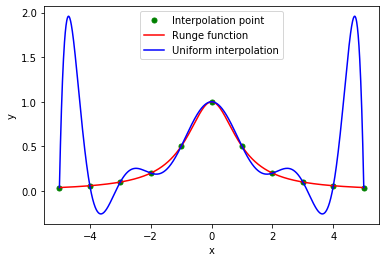
\includegraphics[scale=0.8]{runge.png}
    \caption{Runge's phenomenon. Interpolation with 11 equally spaced nodes. }
\end{figure}
It can be shown that the interpolation will diverge at around $3.63$ as $n\to \infty$ and the maximum error $\max_{x\in[-5, 5]} |f_n(x) - h(x) |$ grows exponentially, where $f_n$ is the interpolating polynomial with $n+1$ equally spaced nodes. In the next section, we outline the idea explaining the phenomenon briefly. 
\subsection{Interpolation Remainder Theory}
\label{SSec: 2-Int-Rem-The}
Let $f_n$ be the degree-$n$ polynomial interpolates $h$ at nodes $\{x_j\}_{j=0}^n$. If $h$ is analytic in a domain $T$ (possibly contains holes),  then the interpolation (Lagrange interpolant) can be written as 
\begin{eqnarray}
    f_n(z) = \sum_{j=0}^n \frac{\omega(z) h(x_j)}{(z - x_j) \omega'(x_j)}
\end{eqnarray}
Let $\psi(\xi; z) = \frac{(\omega(\xi) - \omega(z)) h(\xi)}{(\xi - z) \omega(\xi)}$, then by the Residue theorem for simple poles, if $z \neq x_j$,  
\begin{equation}
    \frac{1}{2\pi i}\int_{\partial T} \psi(\xi; z) d\xi = \sum_{j=0}^n \mathrm{Res}(\psi, x_j) = \sum_{j=0}^n \frac{(\omega(x_j) - \omega(z)) h(x_j)}{(x_j - z)\omega'(x_j)} = f_n(z),
\end{equation}
which implies that 
\begin{equation}
    h(z) - f_n(z) = \frac{1}{2\pi i}\int_{\partial T} \frac{\omega(z) h(\xi)}{(\xi - z)\omega(\xi)} d\xi.
\end{equation}
The error analysis is mainly studying the behavior of $|\omega(z)|$ as $n\to \infty$.
\begin{lemma}
\label{Lem: 2-Ome-Lim}
    If $\{x_j\}_{j=0}^n$ are equispaced nodes over $[a, b]$, then 
    \begin{equation}
        \lim_{n\to\infty} |\omega(z)|^{\frac{1}{n+1}} = \exp\left(\frac{1}{b - a}\int_a^b \log|z-\xi| d\xi \right).
    \end{equation}
\end{lemma}
\begin{proof}
    Taking $\log$ on $|\omega|^{\frac{1}{n+1}}$, then 
    \begin{equation}
        \log |\omega|^{\frac{1}{n+1}} = \frac{1}{n+1}\sum_{j=0}^n \log |z - x_j|\to \frac{1}{b-a}\int_a^b \log|z - \xi| d\xi. 
    \end{equation}
\end{proof}
Let $\sigma_n(z):= |\omega(z)|^{\frac{1}{n+1}}$ and define the contour $C_{\rho} = \{z\in \bbC\mid \sigma_n(z) = \rho\}$. These level sets are concentric closed curves about the midpoint of $[a,b]$.
\begin{lemma}
\label{Lem: 2-Ana-Uni-Con}
    Suppose the interpolation nodes $\{x_j\}_{j=0}^n$ are enclosed by $C_{\rho}$ and $h$ is analytic inside $C_{\rho}$. Let $z\in C_{\rho'}$ be such that $\rho'<\rho$, then $f_n\to h$ uniformly as $n\to\infty$. 
\end{lemma}
\begin{proof}
    Using the maximum modulus principle, the analytic function $h - f_n$ must attain its maximum modulus at the boundary $C_{\rho}$, thus 
    \begin{equation}
        |h(z) - f_n(z)| = \frac{1}{2\pi}\sup_{z\in C_{\rho'}} \left|\int_{C_{\rho}} \frac{\omega(z)}{\omega(\xi)} \frac{h(\xi)}{(\xi - z)} d\xi\right| \le C(\rho, \rho') \sup_{\xi\in C_{\rho}} \frac{|\omega(z)|}{|\omega(\xi)|},
    \end{equation}
    where $C(\rho, \rho')$ is a positive constant independent of $n$. For $n$ sufficiently large, we can find $0 < \delta < \frac{1}{3}(\rho - \rho')$ sufficiently small such that 
    \begin{equation}
        \sup_{\xi\in C_{\rho}} \frac{|\omega(z)|}{|\omega(\xi)|} \le \left|\frac{\rho' + \delta}{\rho - \delta}\right|^{n+1} \to 0\; \text{ as }n\to \infty. 
    \end{equation}
\end{proof}
When $h$ is not analytic inside $C_{\rho}$, let us consider a generic situation in which there exist isolated simple poles $z_k\in C_{\rho_k}$, $k\in [m]$ with $\rho_k < \rho$, then we select a contour $C_{\rho'}$ that $\rho_k <\rho'<\rho$ for all $k$. For $z\in C_{\rho'}$, we have
\begin{equation}
\begin{aligned}
    h(z) - f_n(z) &= \frac{1}{2\pi i} \int_{C_{\rho} - \bigcup_{k=1}^m \Gamma_k} \frac{\omega(z)h(\xi)}{(\xi - z) \omega(\xi)} d\xi \\
    &= \frac{1}{2\pi i} \int_{C_{\rho}} \frac{\omega(z)h(\xi)}{(\xi - z) \omega(\xi)} d\xi - \frac{1}{2\pi i}\sum_{k=1}^m \int_{\Gamma_k}  \frac{\omega(z)h(\xi)}{(\xi - z) \omega(\xi)} d\xi, 
\end{aligned}
\end{equation}
where $\Gamma_k$ is a small path surrounding $z_k$. The first term can be estimated using the lemma~\ref{Lem: 2-Ana-Uni-Con} whose limit goes to zero as $n\to \infty$. The second term is the summation
\begin{equation}
    \sum_{k=1}^m \frac{\omega(z)}{\omega(z_k)}\frac{\mathrm{Res}(h, z_k)}{z_k - z}.
\end{equation}
Since for sufficiently large $n$, we can find $0<\delta<\min_{k\in[m]}\frac{1}{3}(\rho'-\rho_k)$, 
\begin{equation}
    \left|\frac{\omega(z)}{\omega(z_k)}\right|^{\frac{1}{n+1}} = \frac{\sigma_n(z)}{\sigma_n(z_k)} > \min_{k\in [m]}\frac{\rho'-\delta}{\rho_k + \delta} > 1.
\end{equation}
Define the unique set $\cU = \{u_1, u_2,\cdots, u_l\}$ that $u_1 < u_2<\cdots < u_l$ which consists of all distinct values from $\{ \rho_1, \rho_2, \cdots,  \rho_m\}$, then the summation can be decomposed into $l$ groups:
\begin{equation}
 \sum_{k=1}^m \frac{\omega(z)}{\omega(z_k)}\frac{\mathrm{Res}(h, z_k)}{z_k - z} = \sum_{s=1}^l \sum_{\substack{k\in [m] \\ \rho_k = u_s}} \frac{\omega(z)}{\omega(z_k)}\frac{\mathrm{Res}(h, z_k)}{z_k - z}.
\end{equation}
As $n\to\infty$, if any of the groups does not vanish, then the whole summation must blow up as $n\to\infty$ (why?). Otherwise, the limiting summation should vanish which violates the maximum modulus principle. 

In Runge's example~\eqref{EQ: RUNGE-EXAMPLE}, the simple poles $\pm i$ are on the contour $C_{\rho}$ which intersects the real line at $x_c\approx 3.6334$. Therefore for $|x| < x_c$, the interpolation $f_n$ uniformly converges to $h$ and diverges once $|x| > x_c$. See Figure~\ref{fig:contour-curve}.
\begin{figure}[!htb]
    \centering
    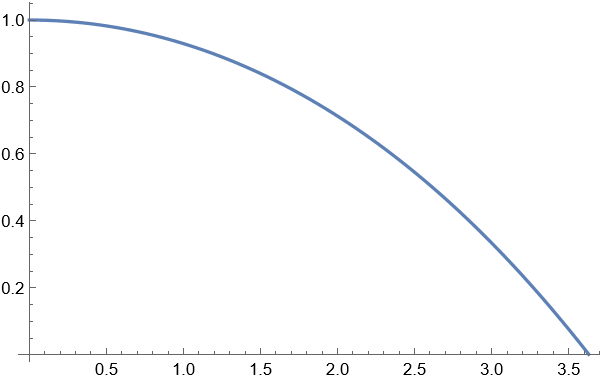
\includegraphics[scale=0.65]{Figures/contour-curve.png}
    \caption{Countour $C_{\rho}$ with $\rho \approx 2.46879$, which passes through the simple pole $i$.}
    \label{fig:contour-curve}
\end{figure}
There exist better choices of interpolation nodes to prevent such a phenomenon. We will discuss this topic in Section~\ref{Sec: 2-Che-Int}. 

\subsection{Chebyshev Interpolation}
\label{Sec: 2-Che-Int}
The Chebyshev interpolation aims to minimize the bound of the interpolation error. The bound of $\omega(x)$ depends only on the choice of the nodes, so a natural question is: What kind of interpolation nodes will \emph{minimize} 
$\max_{x\in [a, b]} \prod_{j=0}^n |x-x_j|$. We first restrict our analysis to the interval $[a, b] = [-1,1]$ for simplicity, the general case will be discussed later.
 
\begin{example}
    When $n = 1$, $\omega(x) = (x - x_0)(x - x_1)$, this function changes sign over the subintervals $[-1, x_0)$, $(x_0, x_1)$, $(x_1, 1]$, then we can compute the maximum of $|\omega(x)|$ on these subintervals. Therefore we need to solve 
    \begin{equation}
        \min_{x_0, x_1\in [-1,1]}\max((1 + x_0)(1 + x_1), \frac{(x_1-x_0)^2}{4}, (1 - x_0)(1 - x_1) ),
    \end{equation}
    while we can observe that 
    \begin{equation}
       \frac{1}{2} (1 + x_0)(1 + x_1) +  \frac{(x_1-x_0)^2}{4} + \frac{1}{2}(1 - x_0)(1 - x_1) = 1 + \frac{(x_0 + x_1)^2}{4}\ge 1
    \end{equation}
    holds for any choice of $x_0, x_1$, which means the maximum is at least $\sfrac{1}{2}$, it occurs when all terms are equal and $x_0 + x_1 = 0$. Hence $x_0 = -\sfrac{\sqrt{2}}{2}, x_1 = \sfrac{\sqrt{2}}{2}$.
\end{example}

\begin{definition}
    The Chebyshev polynomials of the first kind are defined by: 
    $$T_k(x) = \cos (k\arccos x),\quad x\in[-1,1].$$
\end{definition}
\begin{theorem}
\label{Thm: 2-Che-Pro}
    The Chebyshev polynomial satisfies the following: 
    \begin{enumerate}
        \item $T_k(\cos\theta) = \cos k\theta, \quad \theta\in [0, \pi]$.
        \item $T_0 \equiv 1$, $T_1(x) = x$ and 
        $$T_{k+1}(x) = 2 x T_{k}(x) - T_{k-1}(x), \quad k\ge 1.$$
        \item $\max_{x\in[-1,1]} |T_k(x)| = 1$.
        \item The leading coefficient of $T_k(x)$ is $2^{k-1}$.
        \item $T_k$ has a total of $(k+1)$ extrema $s_j = \cos(\frac{j\pi}{k}), j = 0, 1,\dots, n$ in the interval $[-1,1]$ such that $T_k(s_j) = (-1)^j$.
    \end{enumerate}
\end{theorem}
\begin{proof}
    The first three statements are straightforward after replacing the variable $x = \cos\theta$. The fourth statement is an immediate result with induction through the recursion formula 
    $T_{k+1}(x) = 2 x T_k(x) - T_{k-1}$. The last statement is trivial.
\end{proof}
More importantly, the Chebyshev polynomial has the following optimality property. 
\begin{theorem}
\label{Thm: 2-Che-opt}
    The optimal choice of interpolation nodes $\{x_j\}_{j=0}^{n}$ that minimize $\max |\omega(x)|$ is the extrema of Chebyshev polynomial $T_{{n+1}}$.
    \begin{equation}\label{EQ: CHEBY}
        \min_{x_j\in[-1,1]} \max_{x\in[-1,1]} |\omega(x)| =   \max_{x\in[-1,1]} \frac{1}{2^n}|T_{n+1}(x)|  = \frac{1}{2^n}
    \end{equation}
\end{theorem}
\begin{proof}
    Let the roots of $T_{n+1}(x)$ be $z_0, z_1, \dots, z_{n}\in [-1, 1]$, then we can write 
    $$T_{n+1} = 2^{n}(x - z_0)(x-z_1)\dots (x - z_{n}),$$
    therefore $\frac{1}{2^n} T_{n+1}(x)$ is a polynomial with leading coefficient as $1$. Since $\max_{x\in[-1,1]} |T_{n+1}(x)| = 1$, it is clear that $\max_{x\in [-1,1]} \frac{1}{2^n}|T_{n+1}(x)| = \frac{1}{2^n}$, which is the second equality in~\eqref{EQ: CHEBY}. For the first equality, we try to prove it by contradiction. Let $x_0, x_1, \dots, x_n\in [-1, 1]$, such that 
    $$\max_{x\in[-1,1]}|\omega(x)| < \frac{1}{2^n},$$
    then we define the polynomial $\psi(x) = \frac{1}{2^n}T_{n+1}(x)- \omega(x)$, its degree is at most $n$ due to cancellation, therefore at most have $n$ zeros. On the other hand, because $\frac{1}{2^n}T_{n+1}(s_j) = \frac{1}{2^n}(-1)^j$ at the extrema $s_j = \cos(\frac{j\pi}{n+1})$, $j=0,\dots, (n+1)$, the polynomial $\psi(s_j)$ must share the same sign of $\frac{1}{2^n}T_{n+1}(s_j)$. This means $\psi(x)$ changes sign $(n+1)$ times, hence $(n+1)$ zeros. It is a contradiction.
\end{proof}
\begin{definition}
    The interpolation nodes $z_j = \cos(\frac{(2j+1)\pi}{2(n+1)})$, $j = 0, 1, \dots, n$ are called ``\textit{Chebyshev nodes}''. These nodes are the zeros of Chebyshev polynomial $T_{n+1}$.
\end{definition}
We can generalize the above theorem to any interval $[a, b]$. One can defined the affine transformation $\phi$ mapping $[-1,1]$ to $[a, b]$ by $\phi(x) = \frac{1}{2} (a + b + (b-a)x)$. It is not difficult to prove the following.
\begin{corollary}
\label{Cor: 2-Che-err-any}
    The optimal choice of interpolation nodes that minimize $\max |\omega(x)|$ on $[a, b]$ are $\phi(z_j)$ and 
   $$\min_{x_j\in [a, b]} \max_{x\in [a, b]} |\omega(x)| = \frac{(b-a)^{n+1}}{2\cdot 4^n}.$$
   This bound is much smaller than the bound for equally spaced nodes.
\end{corollary}

\subsection{Stability of Polynomial Interpolation}
\label{SSec: 2-Sta-Pol-Int}
Suppose there is some perturbation of the data $\tilde{y}_j = y_j + \eps_j$ at the interpolation node $x_j$. Let $\tilde{f}_n(x)$ and $f_n(x)$ be the interpolating polynomials on perturbed data and original data. Then with Lagrange polynomials, 
\begin{equation}
    \begin{aligned}
        |f_n(x) - \tilde{f_n}(x)| &= |\sum_{j=0}^n (y_j - \tilde{y}_j) L_j(x)| \\
        &\le \left(\max_{j} |\eps_j|\right) \sum_{j=0}^n |L_j(x)|.
    \end{aligned}
\end{equation}
Here $\lambda_n(x) := \sum_{j=0}^n |L_j(x)|$ is the \emph{Lebesgue function}. It is a piecewise-defined polynomial. Its maximum $\Lambda_n$ is the \emph{Lebesgue constant} and only depends on the choice of interpolation nodes. 
For the equally spaced nodes, this Lebesgue constant grows exponentially. 
\begin{lemma}
    \label{Lem: 2-Leb-Con}
    Let $\{x_j\}_{j=0}^n$ be equispaced nodes on $[0, 1]$, then the  Lebesgue constant 
    \begin{equation}
        \frac{2^{n-2}}{n^2} \le \Lambda_n \le \frac{2^{n+3}}{n}.
    \end{equation}
\end{lemma}
\begin{proof}
    Let $f(x) = e^{in\pi x}$,
\end{proof}
In fact,~\cite{turetskii1940bounding} proved a sharper estimate
\begin{equation}
    \Lambda_{n, \textrm{equal}} \sim \frac{2^{n+1}}{en \log n}.
\end{equation}
For the general case, it has been proved by Paul Erd\"os (1964) that there exists a constant $C > 0$
\begin{equation}
    \Lambda_n > \frac{2}{\pi}\log(n+1) - C,\quad  n\ge 0.
\end{equation}
As the number of nodes $n\to \infty$, $\Lambda_n \to \infty$. This leads to the result of Faber that for any choice of nodes, there exists a continuous function not able to be approximated by the interpolating polynomial. The Chebyshev nodes are almost optimal in the sense that 
\begin{equation}
    \Lambda_{n, \textrm{Chebyshev}} < \frac{2}{\pi}\log(n+1) + 1.
\end{equation}
The set of nodes that minimizes $\Lambda_n$ is difficult to compute. A slightly better set of nodes than Chebyshev nodes is the \emph{extended Chebyshev nodes}:
\begin{equation}
    \tilde{x}_j = \frac{\cos\left(\frac{2j+1}{2(n+1)\pi}\right)}{\cos\left(\frac{\pi}{2(n+1)}\right)}.
\end{equation}
\subsection{Newton Form}
The Newton form is useful when we dynamically add interpolation nodes. Consider the following scenario: we already have found an interpolation polynomial $f_k$ through the data $(x_0, y_0)$, $(x_1, y_1)$,$\dots$, $(x_k, y_k)$, then if an addition pair $(x_{k+1}, y_{k+1})$ is provided, how to effectively transform $f_k$ to $f_{k+1}$? If we write 
$$f_{k+1}(x) = f_k(x) + c_{k+1} (x - x_0)(x - x_1)\dots (x - x_{k}), $$
then $f_{k+1}(x_j) = f_k(x_j)$, $j = 0, 1,\dots, k$. Therefore we only need to take care of the equality $f_{k+1}(x_{k+1}) = y_{k+1}$, which means 
\begin{equation}\label{EQ: CK}
    c_{k+1} = \frac{y_{k+1} - f_k(x_{k+1})}{\prod_{j=0}^k (x_{k+1} - x_j)}.
\end{equation}
Such an inductive procedure produces the Newton form: 
\begin{equation}\label{EQ: NEWTON}
    f_n(x) = c_0 + c_1 ( x - x_0) + c_2 (x - x_0)(x - x_1)+\dots+c_{n}(x-x_0)\dots (x - x_{n-1}).
\end{equation}
where the constant $c_j$ depends on $x_0, x_1, \dots, x_{j}$ only. The polynomials $\prod_{j=0}^k (x - x_j)$ are called \emph{Newton polynomials}. When the coefficients $c_k$ are known, the Newton form~\eqref{EQ: NEWTON} can be evaluated by the famous ``Horner's scheme'' (see Exercise~\ref{Prb: 1-Theo-3}), which is
\begin{equation}\label{EQ: HORNER}
    f_n(x) = c_0 + (x-x_0)(c_1 + (x-x_1)(c_2 + (x-x_2)(c_3 + \dots))),
\end{equation}
the evaluation order starts from the innermost part $c_n (x -x_{n-1})$. This formulation has a complexity of $3n$ flops. 

\begin{remark}
    The computation of $c_k$ is not cheap from~\eqref{EQ: CK}. A naive algorithm with Horner's scheme roughly takes $\sfrac{5n^2}{2}+\cO(n)$ flops to compute all coefficients. The ``divided differences'' is a better way to compute $c_k$.
\end{remark}
\begin{definition}
    Let the interpolation nodes be $\{x_0, x_1, \dots, x_n\}$, the ``{divided differences}'' are defined recursively as follows (the square bracket is used to distinguish from the usual bracket): 
    \begin{equation}
        \begin{aligned}
            f[x_j] &:= f(x_j),\\
        f[x_{j}, \dots, x_{j+k}] &:= \frac{f[x_{j+1},\dots, x_{j+k}] - f[x_j,\dots, x_{j+k-1}]}{x_{j+k} - x_{j}},
        \end{aligned}
    \end{equation}
    where $0\le j, k\le n$ and $j+k\le n$.
\end{definition}
The following example graph helps understand the relationships among the divided differences. 

\begin{tcolorbox}
    \begin{equation}\label{EQ: ALG NEWTON}
    \begin{aligned}
        f[x_0] &               &\\ 
               &\searrow       &\\ 
        f[x_1] &\to f[x_0, x_1]& \\
               &\searrow        &\searrow&\\ 
        f[x_2] & \to f[x_1, x_2]&\to& f[x_0, x_1, x_2]\\
               &\searrow        &\searrow& &\searrow&\\ 
        f[x_3] &\to f[x_2, x_3] &\to& f[x_1, x_2, x_3] &\to & f[x_0, x_1, x_2, x_3]\\
               &\searrow        &\searrow & &\searrow&  &\searrow &\\ 
        f[x_4] & \to f[x_3, x_4]&\to& f[x_2, x_3, x_4] &\to & f[x_1, x_2, x_3, x_4] &\to&  f[x_0, x_1, x_2, x_3, x_4] 
    \end{aligned}
\end{equation}
\end{tcolorbox}
Computing all of the divided differences requires $\sfrac{3n^2}{2} +\cO(n)$ flops. The following theorem is the main statement for the Newton form.
\begin{theorem}
\label{Thm: 2-New-for}
    The interpolation polynomial $f_n$ in Newton form is given by 
    \begin{equation}
        f_n(x) = f[x_0] + f[x_0, x_1](x-x_0) + \dots + f[x_0, \dots, x_n](x - x_0)(x - x_1)\dots (x - x_{n-1}).
    \end{equation}
    In other words, $c_k = f[x_0, \dots, x_k]$.
\end{theorem}
\begin{proof}
    We prove this by induction. Assume the statement is true for $n$ and interpolation node and corresponding values $(x_0, f[x_0]), (x_1, f[x_1]), \dots, (x_n, f[x_n])$. For a new node and value $(x_{n+1}, f[x_{n+1}])$, it is known from~\eqref{EQ: CK} that $c_{n+1}$ is the coefficient of leading power. Let $g_n$ be the interpolation polynomial in Newton form through nodes $(x_1, f[x_1]), \dots, (x_{n+1}, f[x_{n+1}])$, then 
    $$\psi(x)  := g_n(x)(x - x_0) - f_n(x)(x - x_{n+1})$$
    satisfies that $\psi(x_j) = f[x_j](x_{n+1} - x_0)$ for $0\le j\le {n+1}$. Therefore 
    \begin{equation}
        f_{n+1}(x) = \frac{g_n(x)(x - x_0) - f_n(x)(x - x_{n+1})}{x_{n+1} - x_0}.
    \end{equation}
    The leading power's coefficient is then 
    \begin{equation}
        \frac{f[x_1, \dots, x_{n+1}] - f[x_0, \dots, x_n]}{x_{n+1} - x_0} = f[x_0, x_1,\dots, x_{n+1}].
    \end{equation}
\end{proof}
\begin{remark}
    The divided difference $f[x_j, \dots, x_{j+k}]$ is the coefficient of leading power of the interpolating polynomial through $(x_j, f[x_j]), \dots, (x_{j+k}, f[x_{j+k}])$. It can be shown that 
    $$f[x_j, \dots, x_{j+k}] = \frac{1}{k!}f^{(k)}(\xi)$$
    for some $\xi\in [a, b]$. See Exercise~\ref{Prb: 2-Theo-4}.
\end{remark}
\begin{remark}
\label{Rem: 2-New-err}
    The error estimate can be derived as 
    \begin{equation}
        f(x) - f_n(x) = f[x_0, x_1, \dots, x_n, x] (x-x_0)\dots (x - x_n).
    \end{equation}
\end{remark}
\begin{remark}
    The Newton form~\eqref{EQ: NEWTON} does not require distinct nodes. The divided difference can be defined as a limit for repeated nodes:
    \begin{equation}
        f[x_0, x_0] = \lim_{x_1 \to x_0} \frac{f[x_1] - f[x_0]}{x_1 - x_0} = f'(x_0).
    \end{equation}
    Moreover, using Taylor expansion, $f[\underbrace{x_0,\dots, x_0}_{(k+1)\,\text{times}}] = \frac{1}{k!}f^{(k)}(x_0)$. However, in such cases, the divided differences are not possible to be computed if the derivative values are not provided. We will discuss this scenario later in Hermite interpolation polynomial, see Section~\ref{SSec: 2-Her-Pol-Int}.
\end{remark}
\begin{remark}
    The algorithm to compute the divided difference can be made more efficient with a single column to store the diagonal elements. $\leadsto$ represents the number that is not changing.
    \begin{tcolorbox}
        \begin{equation}
        \begin{aligned}
            \color{red}{f[x_0]} &    \leadsto  \color{green}{f[x_0]}          & \leadsto& \color{cyan}{f[x_0]} &\leadsto& \color{blue}{f[x_0]} &\leadsto& \color{black}{f[x_0]}\\ 
                   &\searrow       &\\ 
                   \color{red}{f[x_1]} &\to \color{green}{f[x_0, x_1]}&  \leadsto& \color{cyan}{f[x_0, x_1]}  &\leadsto& \color{blue}{f[x_0, x_1]} &\leadsto& \color{black}{f[x_0, x_1]}\\
                   &\searrow        &\searrow&\\ 
                   \color{red}{f[x_2]} & \to \color{green}{f[x_1, x_2]}&\to& \color{cyan}{f[x_0, x_1, x_2]} &\leadsto& \color{blue}{f[x_0, x_1, x_2]}&\leadsto& \color{black}{f[x_0, x_1, x_2]}\\
                   &\searrow        &\searrow& &\searrow&\\ 
                   \color{red}{f[x_3]} &\to \color{green}{f[x_2, x_3] }&\to& \color{cyan}{f[x_1, x_2, x_3]} &\to & \color{blue}{f[x_0, x_1, x_2, x_3]}&\leadsto& \color{black}{f[x_0, x_1, x_2, x_3]}\\
                   &\searrow        &\searrow & &\searrow&  &\searrow &\\ 
                   \color{red}{f[x_4]} & \to \color{green}{f[x_3, x_4]}&\to& \color{cyan}{f[x_2, x_3, x_4]} &\to & \color{blue}{f[x_1, x_2, x_3, x_4]} &\to&  f[x_0, x_1, x_2, x_3, x_4] 
        \end{aligned}
    \end{equation}
    \end{tcolorbox}
\end{remark}
% \subsection{Berstein Polynomial Interpolation}
% The Berstein basis polynomial is defined by 
% \begin{equation}
%     b_{\nu, n}(x) = \binom{n}{\nu} x^{\nu}(1-x)^{n-\nu},\quad  \nu = 0,\dots, n
% \end{equation}

\subsection{Hermite Polynomial Interpolation}
\label{SSec: 2-Her-Pol-Int}
The Lagrange polynomial interpolation only requires the values of the data function $h$ at each node. It can be generalized when the derivative values of $h$ are also available. 

Let the tuple $(h(x_j), h^{(1)}(x_j), \dots, h^{(m_j)}(x_j))$ be the provided derivative values at the interpolation node $x_j$, $j=0,\dots, n$ and $m_j\ge 0$. $N = \sum_{j=0}^n (m_j + 1)$ is the total number of constraints. It can be shown that there exists a unique polynomial $H_{N-1}\in \Pi_{N-1}$ satisfies 
$$H_{N-1}^{(k)}(x_j) = y_j^k:= h^{(k)}(x_j),\quad j=0,\dots, n,\quad 0\le k\le m_j.$$
This polynomial is called \emph{Hermite interpolation polynomial}. The idea to construct the Hermite interpolation polynomial borrows from the Lagrange polynomials, which is to find basis $L_{jk}$ such that 
\begin{equation}\label{EQ: HERMITE CONSTRUCTION}
    \frac{d^p}{d x^p}L_{jk}(x_l) = \begin{cases}
        1, & l = j, k = p\\
        0, & \text{otherwise}.
    \end{cases}
\end{equation}
Once these polynomials are obtained, the Hermite interpolation is straightforward:
$$H_{N-1}(x) = \sum_{j=0}^n \sum_{k=0}^{m_j} y_j^k L_{jk}(x).$$
Its uniqueness can be concluded from the linear independence of the basis $L_{jk}$. However, the construction method in~\eqref{EQ: HERMITE CONSTRUCTION} is not the simplest. It is known that the Newton form~\eqref{EQ: NEWTON} works for repeated nodes as long as the diagram's diagonal~\eqref{EQ: ALG NEWTON} can be filled. Therefore, we can arrange the nodes 
$$\underbrace{x_0,\dots, x_0}_{(m_0+1)\,\text{times}}, \quad \underbrace{x_1,\dots, x_1}_{(m_1+1)\,\text{times}}, \quad \dots,\quad  \underbrace{x_n,\dots, x_n}_{(m_n+1)\,\text{times}}$$
In this way, all of the necessary divided differences can be computed.
\begin{remark}
    The error estimate for Hermite polynomial interpolation will be the same as the Newton form, see Remark~\ref{Rem: 2-New-err}.
\end{remark}


\section{Trigonometric Interpolation}
\label{Sec: 2-Tri-Int}
Periodic functions occur in many applications, that is, $f(x + T) = f(x)$, $x\in \bbR$ for some $T > 0$. For example, a closed planar curve can be parameterized as a periodic function naturally. The polynomial interpolation does not suit periodic functions, this is because polynomials will eventually go to infinity as $x\to\infty$. The most used interpolation for the periodic function is the \emph{trigonometric polynomial interpolation}. In the following, we assume the period $T = 2\pi$ without loss of generality.



\subsection{Fourier Series}
\label{SSec: 2-Fou-Ser}
\begin{definition}
    For $n\ge 0$, we defined $F_n$ the space of trigonometric polynomials 
    \begin{equation}
        F_n := \{f(x) \mid f(x) = \frac{a_0}{2} + \sum_{k=1}^n a_k \cos kx + \sum_{k=1}^n b_k \sin kx,\; a_k, b_k\in\bbR\}.
    \end{equation}
    The coefficients $a_0,\dots, a_n$, $b_1,\dots, b_n$ can be also chosen as complex numbers. $f\in F_n$ is said to be of degree $n$ if $|a_n| + |b_n| > 0$.
\end{definition}
The concept of ``degree'' here can be validated by the addition theorem of trigonometric functions. For instance, if $f_1\in F_k$, $f_2\in F_l$, then $f_1 f_2 \in F_{k+l}$. In the next, we discuss the uniqueness of the interpolation with the trigonometric polynomial.
\begin{lemma}
\label{Lem: 2-Tri-pl-zer}
    A trigonometric polynomial $f\in F_n$ that has more than $2n$ zeros in $[0, 2\pi)$ must vanish identically.
\end{lemma}
\begin{proof}
    Rewrite the trigonometric function in the form of 
    \begin{equation}\label{EQ: COMPLEX}
        f_n(x) = \sum_{k=-n}^{n} \gamma_k e^{ik x}. 
    \end{equation}
    where $\gamma_0 = \frac{1}{2}a_0$ and $\gamma_{k} = \frac{1}{2}(a_k - ib_k)$ and $\gamma_{-k} = \frac{1}{2}(a_k + i b_k)$, $k=1,\dots, n$. Then substitute $z = e^{ix}$ and set 
    \begin{eqnarray}
        p(z) = \sum_{k = -n}^n \gamma_k z^{n + k}, 
    \end{eqnarray}
    one can rewrite $f_n(x) = z^{-n} p(z)$. If $f_n(x)$ has more than $2n$ zeros, then $p(z)$ has more than $2n$ zeros, which is a contradiction since $p(z)$ is a polynomial of degree $2n$.
\end{proof}
\begin{remark}
    Since $\sin nx\in F_n$ has $2n$ zeros $\frac{\pi j}{n}$, $j=0,\dots, 2n-1$, it means to uniquely determine a trigonometric polynomial in $F_n$, exactly $2n+1$ values are needed. This is also known as the ``Nyquist-Shanon sampling theorem''.
\end{remark}
A direct corollary is the linear independence of the functions $1$, $\cos k x$ and $\sin k x$, $k = 1, \dots n$, these $(2n+1)$ functions form a natural basis for the trigonometric polynomial space $F_n$. 
\begin{corollary}
\label{Cor: 2-Fou-bas-ind}
    The functions $1, \cos kx, \sin kx$, $k=1,\dots, n$ are linearly independent on $C [0, 2\pi]$, hence $F_n$ is a $(2n+1)$ dimensional space.
\end{corollary}
To determine the coefficients $a_k, b_k$ from $(2n+1)$ data pairs $(x_j, y_j)$, $j=0, \dots, 2n$. We simply follow the idea of Lagrange polynomials by creating the basis polynomial $l_k(x)$ such that
\begin{eqnarray}
    l_k(x_j) = \begin{cases}
        1, &j = k,\\
        0,&\text{otherwise}.
    \end{cases} 
\end{eqnarray}
\begin{remark}
    A natural idea is replace $x - x_j$ in the Lagrange basis by $\sin(x - x_j)$ and produce something like 
$$\prod_{j=0, j\neq k}^{2n}\frac{\sin(x - x_j)}{\sin(x_k - x_j)}$$
but $\sin(x - x_j)$ has two roots on $[0, 2\pi)$, therefore we need to rescale it to $[0, \pi)$.
\end{remark}
\begin{theorem}
\label{Thm: 2-Tri-Lag}
    Let the basis trigonometric polynomial 
    $$l_k(x) =\prod_{j=0, j\neq k}^{2n}\frac{\sin(\frac{x - x_j}{2})}{\sin(\frac{x_k - x_j}{2})} ,$$
    then the interpolation trigonometric polynomial is 
    \begin{eqnarray}
        f_n(x) = \sum_{k=0}^{2n} y_k l_k(x).
    \end{eqnarray}
\end{theorem}
\begin{proof}
    It remains to show $l_k\in F_n$. This can be seen by splitting $l_k$ into $n$ pairs, each pair takes the form of 
    \begin{eqnarray}
        \sin(\frac{x-x_0}{2})\sin(\frac{x-x_1}{2}) = \frac{1}{2}\cos\left( \frac{x_0 - x_1}{2}\right) - \frac{1}{2}\cos\left(\frac{2x - x_0 - x_1}{2}\right)\in F_1.
    \end{eqnarray}
\end{proof}
Computationally, we can reuse the previously known barycentric form but there exist better methods. For simplicity, we consider the equal space nodes in the following (non-uniform nodes could achieve the same complexity though). 
\begin{eqnarray}
    x_j = \frac{2\pi j}{2n + 1}, \quad j = 0, \dots, 2n. 
\end{eqnarray}
We will try to locate the coefficients $\gamma_k$ in the complex form (see~\eqref{EQ: COMPLEX}) from the interpolation conditions.
\begin{equation}
    f_n(x_j) = y_j = \sum_{k=-n}^n \gamma_k e^{i k x_j}.
\end{equation}
Use the property of the functions $e^{ikx_j}$ that 
\begin{equation}
    \sum_{k=0}^{2n} e^{ik x_j} = \begin{cases}
        2n+1, & k = 0\\
        0, &\text{otherwise}.
    \end{cases}
\end{equation}
It is not difficult to derive 
\begin{equation}
    \sum_{j = 0}^{2n} y_j e^{-im x_j} = \sum_{k=-n}^{n} \gamma_k \sum_{j=0}^{2n} e^{i (k - m) x_j} = \gamma_{m} (2n+1).  
\end{equation}
Therefore, we can compute 
\begin{equation}\label{EQ: GAMMA}
    \gamma_m = \frac{1}{2n+1}  \sum_{j = 0}^{2n} y_j e^{-im x_j}.
\end{equation}
When the coefficients $\gamma_m$ are known, Horner's scheme can be employed to evaluate the trigonometric polynomial in $\cO(n)$ time complexity.  However, naive computing of all of the coefficients $\gamma_k$ will cost $\cO(n^2)$ flops. The fast Fourier transform can reduce the time complexity to $\cO(n\log n)$.
\begin{remark}
    For even number of equally spaced nodes $x_j = \frac{j\pi}{n}$, $0\le j\le 2n-1$, the basis $\sin( n x)$ equals to zero constantly. There are $2n$ coefficients to be determined only. We can derive a similar formula as~\eqref{EQ: GAMMA} by replacing $(2n+1)$ with $2n$.
\end{remark}

\subsection{Fast Fourier Transform}
\label{SSec: 2-Fas-Fou-Tra}
The discrete Fourier transform $\textup{\texttt{DFT}}$ of a vector $\ba = (a_0, \dots, a_{n-1})$ is to evaluate the following vector:
$$\textup{\texttt{DFT}}(\ba)_{k} := \frac{1}{n}\sum_{j=0}^{n-1} a_je^{-2\pi i jk/n},\quad k = 0,\dots, n-1.$$
This is the exact formula to compute the coefficients for the trigonometric interpolation polynomial. Such transform is most efficiently calculated through the fast Fourier transform (\texttt{fft}).
The fast Fourier transform exploits the symmetry in $e^{2\pi i j/n}$ when $n$ is the power of two using divide-and-conquer. Let $\omega = e^{-2\pi i/n}$ and define $c_k$ as 
\begin{equation}
    c_k = \frac{1}{n}\sum_{j=0}^{n-1} y_j\omega^{jk},\quad k = 0,\dots, n-1.
\end{equation}
Let $m = \sfrac{n}{2}\in \bbN$, then $\omega^n = 1$, $\omega^m = -1$. We can separate $c_k$ into two parts with even $j$ and odd $j$.
\begin{equation}\label{EQ: C_K}
    c_k = \frac{1}{2} A_k + \frac{1}{2} B_k \omega^k,\quad c_{k+m} = \frac{1}{2} A_k - \frac{1}{2} B_k \omega^k 
\end{equation}
where 
\begin{equation}\label{EQ: AK BK}
    \begin{aligned}
        A_k = \frac{1}{m} \sum_{j=0}^{m-1} y_{2j} (\omega^2)^{jk},\quad B_k = \frac{1}{m} \sum_{j=0}^{m-1} y_{2j+1} (\omega^2)^{jk},
    \end{aligned}
\end{equation}
both $A_k$ and $B_k$ are in the same form and similar to $c_k$, but with only half of the terms in summation. This implies a recursive algorithm. Suppose $A_k$ and $B_k$, $0\le k\le m-1$ can be computed with $f(m)$ operations each, then 
\begin{equation}
   f(n) =  f(2m) = 2 f(m) + 4m
\end{equation}
The second term includes $2m$ multiplications and $2m$ additions in~\eqref{EQ: C_K}. Therefore
\begin{equation}
    \begin{aligned}
        f(n)& = 2f(\frac{n}{2}) + 2n \\
&= 4f(\frac{n}{4}) + 2 n + 2n \\ 
&=\dots \\
&= n f(1) + \underbrace{2n + \dots + 2n}_{\log_2 n \text{ times}} = 2n \log_2 n.
    \end{aligned}
\end{equation}
since $f(1) = 0$, no computation is needed in this case.  The \texttt{fft} is usually a standard routine in modern scientific computing software. 

\subsection{Interpolation Error of Trigonometric Polynomial}
\label{SSec: 2-Int-Err-Tri-Pol}
The $L^2$ error estimate will be discussed at a later point. This part only focuses on the $L^{\infty}$ error estimate. We will need the following lemma, the proof is left as an exercise (see Exercise~\ref{Prb: 2-Theo-6}).
\begin{lemma}
\label{Lem: 2-Dir-Ker}
    Let $g(x)$ be the truncated Fourier series of $f(x)$
     $$g(x) = \sum_{s = -n}^n \gamma_s e^{is x},\quad \gamma_s = \frac{1}{2\pi}\int_{0}^{2\pi} f(x) e^{-isx} dx$$
     then 
     \begin{equation}
         g(x) =\frac{1}{2\pi}  \int_{0}^{2\pi} D_n(x - y) f(y)   d y, 
     \end{equation}
     where $D_n(x)$ is the \emph{Dirichlet kernel}
     \begin{equation}
         D_n(x):=  \sum_{s=-n}^{n} e^{is x} = \frac{\sin((2n+1)x/2)}{\sin(x/2)}.
     \end{equation}
\end{lemma}
\begin{theorem}[Uniform convergence for H\"older continuous functions]
\label{Thm: 2-Uni-Conv-C2}
    If $f\in C^{0,\alpha}(\bbR)$ is a $2\pi$-period function, then the trigonometric interpolation polynomial with $2n+1$ equally spaced nodes converges uniformly as the number of nodes tends to infinity.
\end{theorem}
\begin{proof}
    Let $g(x)$ be the truncated Fourier series
    $$g(x) = \sum_{s = -n}^n \gamma_s e^{is x},\quad \gamma_s = \frac{1}{2\pi}\int_{0}^{2\pi} f(x) e^{-isx} dx$$
   and denote $h(x) = f(x)- g(x) = \sum_{|s| > n} \gamma_s e^{isx}$ the reminder. The interpolation polynomial satisfies
    \begin{equation}
        \begin{aligned}
            f_n(x)& = \sum_{m=-n}^n \left(\frac{1}{2n+1}\sum_{j=0}^{2n} y_j e^{-im x_j}\right) e^{im x}  \\
             &=\sum_{m=-n}^n \left(\frac{1}{2n+1}\sum_{j=0}^{2n} ( g(x_j) + h(x_j) ) e^{-im x_j}\right) e^{im x} \\
             &= \sum_{m=-n}^n \left(\frac{1}{2n+1}\sum_{j=0}^{2n} ( \sum_{s = -n}^n \gamma_s  e^{is x_j }+ h(x_j) ) e^{-im x_j}\right) e^{im x} \\
             &=g(x)+ \sum_{m=-n}^n \left(\frac{1}{2n+1}\sum_{j=0}^{2n} h(x_j) e^{-im x_j}\right)e^{im x} \\
             &=g(x)+ \frac{1}{2n+1} \sum_{j=0}^{2n} h(x_j) \frac{\sin((2n+1)(x-x_j)/2)}{\sin((x-x_j)/2)}
        \end{aligned}
    \end{equation}
    Therefore 
    \begin{equation}\label{EQ: DIFF}
        |f - f_n| \le \|h\|_{\infty} \left( 1 + \frac{1}{2n+1} \sum_{j=0}^{2n} \left|\frac{\sin((2n+1)(x-x_j)/2)}{\sin((x-x_j)/2)}\right|\right).
    \end{equation}
    We first estimate 
    $$\sum_{j=0}^{2n} \left|\frac{\sin((2n+1)(x-x_j)/2)}{\sin((x-x_j)/2)}\right|$$
    Separate the nodes into two groups: The first group with $|x - x_j| < \frac{2\pi}{2n+1}$, the absolute value is bounded by $(2n+1)$, there are at most $3$ nodes lying in this region, thus the contribution from the first group is at most $\cO(n)$. The second group is $\pi\ge |x - x_j| \ge \frac{2\pi}{2n+1}$, then one can estimate 
    \begin{equation}
        \left|\frac{\sin((2n+1)(x-x_j)/2)}{\sin((x-x_j)/2)}\right| \le \frac{\pi}{|x - x_j|},
    \end{equation}
    since $\pi \sin x \ge 2x $ for $0\le x\le \sfrac{\pi}{2}$. This implies the contribution from the second group is $\cO(n\log n)$, and the total contribution is bounded by $\cO(n\log n)$. Then~\eqref{EQ: DIFF} can be bounded by 
    \begin{equation}
        |f - f_n| \le C \|h\|_{\infty} \log n,
    \end{equation}
    where $C$ is an absolute constant. Next, we estimate $\|h\|_{\infty}$. Using Lemma~\ref{Lem: 2-Dir-Ker}, we can represent
    \begin{equation}
    \begin{aligned}
        h(x) &= \frac{1}{2\pi} \int_{-\pi}^{\pi} D_n(y) (f(x) - f(x - y) ) dy \\
        &= \frac{1}{2\pi} \sum_{k=-n}^{n} \int_{\frac{(2k-1)\pi}{2n+1}}^{\frac{(2k+1)\pi}{2n+1}} \frac{\sin((2n+1) y/2)}{\sin(y/2)}  (f(x) - f(x - y) ) dy.
    \end{aligned}
    \end{equation}
    Notice the cancellation property
    \begin{equation}
         \int_{\frac{(2k-1)\pi}{2n+1}}^{\frac{(2k+1)\pi}{2n+1}} \sin\left(\frac{(2n+1) y}{2}\right) dy = 0,
    \end{equation}
    then for any $y'\in \cI_k:= \left(\frac{(2k-1)\pi}{2n+1}, \frac{(2k+1)\pi}{2n+1}\right)$, we have 
    \begin{equation}
    \label{EQ: CANCELLATION F}
    \begin{aligned}
    &\left| \int_{\frac{(2k-1)\pi}{2n+1}}^{\frac{(2k+1)\pi}{2n+1}} \frac{\sin((2n+1) y/2)}{\sin(y/2)}  (f(x) - f(x - y) ) dy \right| \\
    &= \left| \int_{\frac{(2k-1)\pi}{2n+1}}^{\frac{(2k+1)\pi}{2n+1}} \sin((2n+1) y/2)  \left( \frac{(f(x) - f(x - y) )}{\sin(y/2)} - \frac{(f(x) - f(x - y') )}{\sin(y'/2)} \right) dy \right| \\
    &\le \frac{4}{2n+1}\sup_{y,y'\in \cI_k} \left| \frac{(f(x) - f(x - y) )}{\sin(y/2)} - \frac{(f(x) - f(x - y') )}{\sin(y'/2)} \right|\\
    &\le \frac{4K}{2n+1}\left(\frac{\frac{\pi}{2n+1}\left|\frac{(2|k|+1)\pi}{2n+1}\right|^{\alpha}+ \frac{(2|k|+1)\pi}{4n+2}\left|\frac{2\pi}{2n+1}\right|^{\alpha}}{\left|\frac{(2|k|-1)\pi}{4n+2}\right|^2}\right)\\
    &=\frac{8K\pi^{\alpha-1}}{(2n+1)^{\alpha}} \left( \frac{2(2|k|+1)^{\alpha}}{(2|k|-1)^2}+ 2^{\alpha}\frac{2|k|+1}{(2|k|-1)^2} \right).
    \end{aligned}
    \end{equation}
    Because $\left|\frac{2|k|-1}{2|k|+1}\right|\ge \frac{1}{3}$ for all $k\in\bbN$, we obtain the bound for $h$:
    \begin{equation}
    \begin{aligned}
        |h(x)| &\le  \frac{4K\pi^{\alpha-2}}{(2n+1)^{\alpha}} \sum_{k=-n}^{n}  \left( \frac{2(2|k|+1)^{\alpha}}{(2|k|-1)^2}+ 2^{\alpha}\frac{2|k|+1}{(2|k|-1)^2} \right)\\&
        \le  \frac{36K\pi^{\alpha-2}}{(2n+1)^{\alpha}} \sum_{k=-n}^{n}  \left( \frac{2}{(2|k|+1)^{2-\alpha}}+ \frac{ 2^{\alpha}}{(2|k|+1)} \right)\\
        &= \cO(n^{-\alpha} \log n).
    \end{aligned}
    \end{equation}
    Therefore $|f - f_n|=\cO( n^{-\alpha} |\log n|^2 )$.
\end{proof}
\begin{remark}
    This can be further extended to general continuous functions with \emph{modulus of continuity} $\omega(f;\tau)$ satisfying $\omega(f;\frac{1}{n})\log n \to 0$ as $n\to\infty$, see the work of Dunham Jackson (1913). More related topics are discussed in Chapter~\ref{Ch: 4-App}.
\end{remark}

\section{Spline Interpolation}
\label{Sec: 2-Spl-Int}
It has been seen that increasing the number of interpolation nodes will not always help improve the approximation. The spline interpolation is to conquer this issue by using the piecewise low-degree polynomials. 

\begin{definition}
    Let $x_0, \dots, x_n$ be the distinct nodes on $[a, b]$ such that $a = x_0 <\dots < x_n = b$. The piecewise defined function $s_k(x)$ on the interval $[a, b]$ is a spline of degree $k$ to the nodes if  
    \begin{equation}
        s_k|_{[x_j, x_{j+1}]} \in \Pi_k, \quad s_k\in C^{k-1}([a, b]).
    \end{equation}
    The spline function $s_k$ is $(k-1)$-times continuously differentiable and piecewise polynomial of degree $k$.
\end{definition}
Then the space of splines $s_k$ will be $(n + k)$ dimension: each interval has $(k+1)$ dimensions, each interface imposes $k$ constraints, therefore $n (k+ 1) - (n-1) k = n + k$ dimensions. This shows that to determine a spline on the nodes uniquely, we will require $n+1$ interpolation values and $k-1$ additional constraints. Usual choices are
\begin{enumerate}
    \item periodic splines. $s_k^{(m)}(a) = s_k^{(m)}(b)$ for $m = 0, 1, \dots, k-1$.
    \item natural splines. $s_k^{(l+j)}(a) = s_k^{(l+j)}(b) = 0$, $j = 0, 1,\dots, l-2$ and $k = 2l-1$ with $l\ge 2$.
\end{enumerate}
In the following, we discuss some useful examples of spline. 
\subsection{Linear Splines}
The linear splines are a special case of splines. It uses piecewise linear polynomials on each subinterval and does not impose any derivative continuity. Let $y_j$ be the interpolation values at nodes $x_j$, respectively. The interpolation has an explicit form:
\begin{equation}
    s_1(x) = y_{j-1} + \frac{x - x_{j-1}}{x_j - x_{j-1}} y_j
\end{equation}
on the interval $[x_{j-1}, x_j]$. It can be represented as a linear combination of the ``hat'' basis function $\theta_j(x)$, defined by
\begin{equation}
    \theta_j(x) = \begin{cases}
        \frac{x - x_{{j-1}}}{x_j - x_{j-1}}, & x\in [x_{j-1}, x_{j}],\quad 1\le j\le n\\
         \frac{x - x_{j+1}}{x_j - x_{j+1}}, & x\in [x_j, x_{j+1}],\quad 0\le j\le n-1\\
         0, & \text{otherwise}
    \end{cases}
\end{equation}
then $s_1(x)$ can be written as 
$$s_1(x) = \sum_{j=0}^n \theta_j(x) y_j.$$
The interpolation error can be derived directly from the previous theory for two interpolation nodes. Let $f\in C^2([a, b])$, then on $[x_{j-1}, x_j]$, the interpolation error is 
\begin{equation}
    \frac{1}{2!}f''(\xi) (x - x_{j-1})(x - x_j) \le \frac{1}{8} \|f''\|_{\infty} |x_j - x_{j-1}|^2.
\end{equation}
Therefore, the interpolation error on $[a, b]$ is $\frac{1}{8} \|f''\|_{\infty} h^2$, where $h = \max|x_j - x_{j-1}|$. Once $f''$ is not uniformly bounded or even $f'$ is not well-defined somewhere, e.g., $f\in C^{0,\alpha}[a, b]$, the interpolation error will be replaced by the modulus of continuity. On $x\in [x_j, x_{j+1}]$, we have 
\begin{equation}
\begin{aligned}
    |s_1(x) - f(x)| &= \left| \frac{ (x_{j+1} - x) y_j+ (x - x_j) y_{j+1}}{x_{j+1} - x_j} - f(x) \right| \\   
    &=  \left| \frac{ (x_{j+1} - x) (y_j - f(x)) + (x - x_j) (y_{j+1}-f(x))}{x_{j+1} - x_j}  \right| \\ &\le \omega(f; |x_{j+1} - x_j|),
\end{aligned}
\end{equation}
where $\omega(f;\tau)$ is the modulus of continuity of $f$.
\subsection{Cubic Splines}
The cubic splines are particularly important in practice. Let $a = x_0 < x_1 <\dots < x_n = b$, and the corresponding values are $y_j$, $j = 0, \dots, n$. The constraints for cubic splines are: piecewise polynomial of degree 3 and continuous second derivative.a Denote the interpolation spline as $s_3$, then $\dd{s_3}$ is a piecewise linear function. On the sub-interval $[x_{j-1}, x_j]$, it can be represented by 
\begin{equation}
    \dd{s_3}(x) = M_{j-1} \frac{x_j - x}{h_j} + M_j \frac{x - x_{j-1}}{h_j},\quad j = 1,\dots, n,
\end{equation}
where $h_j = x_j - x_{j-1}$, $M_j = \dd{s_3}(x_j)$. Integrating the above formula twice, 
\begin{equation}
    s_3(x) = M_{j-1} \frac{(x_j - x)^3}{6 h_j} + M_j \frac{(x - x_{j-1})^3}{6h_j} + A_j (x - x_{j-1}) + B_j
\end{equation}
The additional constants $A_j, B_j$ can be determined by imposing $f(x_{j-1}) = y_{j-1}$ and $f(x_j) = y_j$. That is 
\begin{equation}
    A_j = \frac{y_j - y_{j-1}}{h_j} - \frac{h_j}{6}(M_j - M_{j-1}),\quad 
    B_j = y_{j-1}-  M_{j-1} \frac{h_j^2}{6}.
\end{equation}
Now we will determine the constants $M_j$ using the first derivative's continuity. 
\begin{equation}
    s_3'(x_{j}^{-})  = s_3'(x_j^{+}), \quad j = 1,\dots, n-1.
\end{equation}
That is equivalent to $j=1,\dots, n-1$, 
\begin{equation}
    \begin{aligned}
        s_3'(x_{j}^{-})  &= M_j\frac{h_j}{3} + M_{j-1}\frac{h_{j}}{6} + \frac{y_j - y_{j-1}}{h_j}  \\
        &= -M_j \frac{h_{j+1}}{3}  - M_{j+1}\frac{h_{j+1}}{6} + \frac{y_{j+1} - y_j}{h_{j+1}} = s_3'(x_j^{+}). 
    \end{aligned}
\end{equation}
We can write the corresponding equations into a tri-diagonal linear system 
\begin{equation}
    \begin{pmatrix}
        \frac{h_1}{6} & \frac{h_1 + h_{2}}{3} & \frac{h_{2}}{6} & \\\\
        &\frac{h_2}{6} & \frac{h_2 + h_{3}}{3} & \frac{h_{3}}{6} & \\\\
        &&\ddots &  \ddots & \ddots & \\ \\
        &&& \frac{h_{n-1}}{6} & \frac{h_{n-1} + h_{n}}{3} & \frac{h_{n}}{6} &
    \end{pmatrix} \begin{pmatrix}
        M_0 \\\\M_1\\\\ \vdots\\\\ M_n
    \end{pmatrix} 
    = \begin{pmatrix}
        \frac{y_{2} - y_{1}}{h_{2}} - \frac{y_{1} - y_{0}}{h_1} \\\\
        \frac{y_{3} - y_{2}}{h_{3}} - \frac{y_{2} - y_{1}}{h_2} \\\\
        \vdots \\\\
        \frac{y_{n} - y_{n-1}}{h_{n}} - \frac{y_{n-1} - y_{n-2}}{h_{n-1}} 
    \end{pmatrix}
\end{equation}
In practice, the system will be rescaled for numerical stability. 
\begin{equation}\nonumber
    \begin{pmatrix}
        \frac{h_1}{2(h_1 + h_{2})} & 1 & \frac{h_{2}}{2(h_1 + h_{2})} & \\\\
        &\frac{h_2}{2(h_2 + h_{3})} & 1 & \frac{h_{3}}{2(h_2 + h_{3})} & \\\\
        &&\ddots &  \ddots & \ddots & \\ \\
        &&& \frac{h_{n-1}}{2(h_{n-1} + h_{n})} & 1 & \frac{h_{n}}{2(h_{n-1} + h_{n})} &
    \end{pmatrix} \begin{pmatrix}
        M_0 \\\\M_1\\\\ \vdots\\\\ M_n
    \end{pmatrix} 
    = \begin{pmatrix}
       d_1 \\\\
        d_2 \\\\
        \vdots \\\\
       d_{n-1}
    \end{pmatrix}
\end{equation}
where $d_j = \frac{3}{h_{j-1} + h_{j}}\left[ \frac{y_{j} - y_{j-1}}{h_{j}} - \frac{y_{j-1} - y_{j-2}}{h_{j-1}}\right]$. 
The above system still lacks 2 more constraints since the matrix is of size $(n-1)\times (n+1)$. Then we can apply the periodic spline or natural spline conditions. For example, if the natural constraint is applied: $\dd{s_3}(a) = \dd{s_3}(b) = 0$. We should have two more equations: 
\begin{equation}
    M_{0} = M_{n} = 0.
\end{equation} 
Then we can simply ignore the first and last columns of the matrix (also $M_0$ and $M_n$). 
If the periodic constraint is imposed, then we can add two more constraints: $M_0 = M_{n}$ and 
$$-M_0 \frac{h_{1}}{3} - M_1 \frac{h_1}{6} + \frac{y_1 - y_0}{h_1} = M_n \frac{h_n}{3} + M_{n-1} \frac{h_n}{6} + \frac{y_n - y_{n-1}}{h_n}.$$
In both cases, the resulting linear system is still tridiagonal and the solution takes $\cO(n)$ time complexity with the Thomas algorithm. 

Another popular choice to complete the matrix is to impose the constraints in the similar form on $x_0$ and $x_n$: 
\begin{equation}
\label{EQ: EXTENSION}
    2M_0 + \frac{h_1}{h_0 + h_1} M_1 = d_0,\quad  \frac{h_n}{h_{n} + h_{n+1}} M_{n-1} + 2M_n = d_n,
\end{equation}
where $h_0 = h_{n+1} = 0$ and $d_0 = d_1$, $d_{n} = d_{n-1}$ are assumed. 
\begin{remark}
The Jacobi and Gauss-Seidel iterations are suitable for solving the system. The iteration will converge to system accuracy within $\cO(\log_2 \textup{u})$ iterations. Related topics are discussed in Chapter~\ref{Ch: 8-Mat-Com}.
\end{remark}
The error estimate for the cubic spline can be derived in a way similar to the Lagrange polynomial interpolation. The following result is attributed to Charles Hall (1968).
\begin{theorem}\label{THM: ERROR CUBIC SPLINE}
    Let $f\in C^4([a, b])$ and $a = x_0 < \dots < x_n = b$ be a set of nodes. Then the natural cubic spline $s_3$ interpolating $f$ satisfies 
    \begin{equation}
        \|f - s_3\|_{\infty} \le \frac{5}{384}\|f^{(4)}\|_{\infty} h^4,
    \end{equation}
    where $h = \max_j |x_j - x_{j-1}|$.
\end{theorem}
\begin{proof}
    Here we only state the rough idea to prove the error bound. Let $u(x)$ be the piecewise-defined Hermite interpolation polynomial that 
    \begin{equation}
        u(x_j)=f(x_j), \quad u'(x_j) = f'(x_j),
    \end{equation}
    then one can estimate 
    \begin{equation}
        \max_{x\in [x_j, x_{j+1}]} |u-f|\le  \frac{1}{24}\|f^{(4)}\|_{\infty} (x - x_j)^2 (x - x_{j+1})^2 \le \frac{1}{384}\|f^{(4)}\|_{\infty} h^4.
    \end{equation}
    Then show that $\|s_3 - u\|_{\infty}$ is bounded by $\cO(\|f^{(4)}\|_{\infty} h^4)$. This step needs to analyze the error $\|s_3' - f'\|_{\infty}$. Todo.
\end{proof}
\subsection{B-Spline Representation}

\section{Reproduce Kernel Hilbert Space}


\section{Exercises}
The coding part and test cases are available on GitHub. 
\subsection{Theoretical Part}
\begin{problem}
    Prove Corollary~\ref{Cor: 2-Che-err-any}.
\end{problem}
\begin{problem}
    If $n$ is sufficiently large, prove the following bound instead for~\eqref{EQ: MAX-OMEGA}.
    \begin{equation}
        |\omega(x)|\le \prod_{j=0}^n |x - x_j| \le \frac{n!}{1 + \log n} \left|\frac{b-a}{n}\right|^{n+1}.
    \end{equation}
\end{problem}
\begin{problem}
\label{Prb: 2-Theo-2}
    Estimate the interpolation error for $e^x$ and $x^{-\sfrac{1}{2}}$ over the interval $[\frac{1}{2}, \frac{3}{2}]$ with equally spaced nodes and Chebyshev nodes, respectively.
\end{problem}
\begin{problem}
    Let $-1\le x_0 < x_1 <\dots < x_n \le 1$ be a set of interpolation nodes and $L_j(x)$ denotes the Lagrange basis polynomial at $x_j$. Prove if $x\in (x_i, x_{i+1})$, then 
    $$L_{i}(x) + L_{i+1}(x) \ge 1.$$
    Hint: Use Rolle's Theorem.
\end{problem}
\begin{problem}
    Prove the contour $C_{\rho}$ for Chebyshev nodes on $[-1, 1]$ is an ellipse with foci at $\pm 1$. 
\end{problem}
\begin{problem}
\label{Prb: 2-Theo-4}
    Let the nodes $x_0, \dots, x_n\in[a,b]$ and $f\in C^{n+1}([a, b])$. For any given $x\in[a, b]$, prove there exists $\xi\in [a, b]$ such that the divided difference $$f[x_0, x_1, \dots, x_n, x] = \frac{1}{(n+1)!}f^{(n+1)}(\xi).$$
    Hint: {Construct the interpolation polynomial on nodes $x_0, \dots, x_n$ with Newton form first, then regard $x$ as the additional node by~\eqref{EQ: NEWTON}, finally recall the Theorem~\ref{Thm: 2-Int-err}.}
\end{problem}
\begin{problem}
    Show that the divided difference $$f[x_0, x_1,\dots, x_n] = f[x_{\pi(0)}, x_{\pi(1)},\dots, x_{\pi(n)}],$$ where $\pi\in S_{n+1}$ is any permutation.
\end{problem}
\begin{problem}
\label{Prb: 2-Theo-6}
    Prove Lemma~\ref{Lem: 2-Dir-Ker}.
\end{problem}
\begin{problem}[discrete circular convolution]
    Let two vectors $\ba = (a_0,\dots, a_{N-1})$ and $\bb = (b_0, \dots, b_{N-1})$ and we assume the convention that $a_{N + j} = a_j$ and $b_{N+j} = b_j$ to extend the vector to infinite size. The discrete circular convolution $\bc = (c_0,\dots, c_{N-1}) = \ba\ast \bb$ is defined by 
$$c_j = \sum_{l = 0}^{N-1} a_l b_{j - l}.$$
Prove that 
$$\textup{\texttt{DFT}}(\bc) = \textup{\texttt{DFT}}(\ba)\circ \textup{\texttt{DFT}}(\bb),$$
where $\circ$ is the Hadamard product or element-wise product.
\end{problem}
\begin{problem}[Minimimum norm property] Let $f\in C^2([a, b])$ and $s_3$ be the \underline{natural} cubic spline with interpolating $f$. Prove 
    \begin{equation}
        \int_a^b |\dd{s_3}(x)|^2 dx \le \int_{a}^b |f''(x)|^2 dx 
    \end{equation}
    The equality holds only when $f(x) = s_3(x)$ everywhere.
    Hint: One needs to prove 
    \begin{equation}
        \int_a^b (f''(x) - \dd{s_3}(x)) \dd{s_3}(x) dx = 0,
    \end{equation}
    then simply use the AM-GM inequality. The above equality can be proved using integration-by-parts twice (remember the interpolation conditions).
\end{problem}
\begin{problem}
    Let the following tri-diagonal matrix (corresponding to natural cubic spline)
    $$A = \begin{pmatrix}
        1 & \frac{h_{2}}{2(h_1 + h_{2})} & \\\\
        \frac{h_2}{2(h_2 + h_{3})} & 1 & \frac{h_{3}}{2(h_2 + h_{3})} & \\\\
        &\ddots &\ddots &  \ddots & \\ \\
        &&\ddots &\ddots &  \frac{h_{n-2}}{2(h_{n-2} + h_{n-1})} & \\ \\
        &&& \frac{h_{n-1}}{2(h_{n-1} + h_{n})} & 1&
    \end{pmatrix} $$
    and denote $B = A - I$. Prove $\|B\|_{\infty} \le \frac{1}{2}$ and $\|A^{-1}\|_{\infty}\le 2$. 
\end{problem}

% \begin{problem}
%     Complete the proof of Theorem~\ref{THM: ERROR CUBIC SPLINE}.
% \end{problem}
\subsection{Computational Part}
\begin{problem}
    Implement the divided difference to compute the coefficients of the Newton form. You should call the Horner's scheme from the previous coding project. State the consequence when the length of $[a, b]$ is very small. 
\end{problem}
\begin{problem}
    Implement the Lagrange interpolation schemes on equispaced nodes and (extended) Chebyshev nodes.
\end{problem}
\begin{problem}
    Implement a routine to compute Hermite interpolation with $m_j = 1$ for each $j = 0, \dots, n$. Estimate your routine's time complexity and space complexity. 
\end{problem}
\begin{problem}
    Implement the cubic spline interpolation with periodic and natural spline conditions. 
\end{problem}

\begin{problem}
     Implement discrete Fourier transform using a recursive approach (assume the total number of nodes is a power of two).
\end{problem}

% \bibliography{563}
\nocite{jackson1912approximation, jackson1913accuracy, erdHos1964problems,erdos1958problems,de1978practical,prenter2008splines}
\bibliographystyle{apalike}
\bibliography{chap2}
